\documentclass[12pt,a4paper]{article}
\usepackage[top=25.4mm, bottom=25.4mm, left=19.1mm, right=19.1mm]{geometry}


\usepackage[latin2]{inputenc}
\usepackage{graphicx}
\graphicspath{ {./images/} }
\usepackage{ulem}
\usepackage{amsmath}
\usepackage[document]{ragged2e}

\setlength{\parindent}{4em}
\setlength{\parskip}{1em}
\usepackage{hyperref}

\usepackage{fancyhdr}
\pagestyle{fancy}
\fancyhf{}
\fancyhead[LO]{\textbf{\small IoT and Smart Analytics}\\
\text{\small A Program by IIITH and TalentSprint}}

\usepackage{xcolor}
\usepackage{lipsum}

\rhead{\begin{picture}(0,0) \put(-250,-2){
\includegraphics[width=9cm]{EXP_06_Images/ts-iisc-logo-pr.png}} \end{picture}}
\cfoot{\thepage}


\begin{document}

\begin{center}

\textbf{\large \\EXPERIMENT 03 }\\[6pt]
\text{ LED blinking with Arduino }
\end{center}

\textbf{\large LEARNING OBJECTIVES:}\\[3pt]
At the end of this experiment, participants will be able to:\vspace{-6mm}\begin{enumerate}
 \setlength\itemsep{-0.3em}
\item Understand input/outputs pins and their applications
\item Understand basic functions: void setup (), void loop (), PinMode(), digitalWrite(), delay()
\item  LED blinking with Arduino in TinkerCAD
\item  Implement LED blinking with Arduino physical hardware

\end{enumerate}
\textbf{\large APPARATUS REQUIRED:}\\
\vspace{-3mm}
\begin{enumerate}
 \setlength\itemsep{-0.3em}
\item A good internet connection
\item Arduino-1
\item Power adapter-1
\item LED-1
\item Resistor 1k$\Omega$-1pcs
\item Breadboard
\item Jumper wires

\end{enumerate}

\begin{justify}
\textbf{\large THEORY}\\[3pt]
To start with Arduino, we will be blinking an LED. This baseline will give you a solid foundation as we work towards experiments that are more complex.  Below is the circuit diagram of LED connection with Arduino Uno board.

    \begin{center} 
    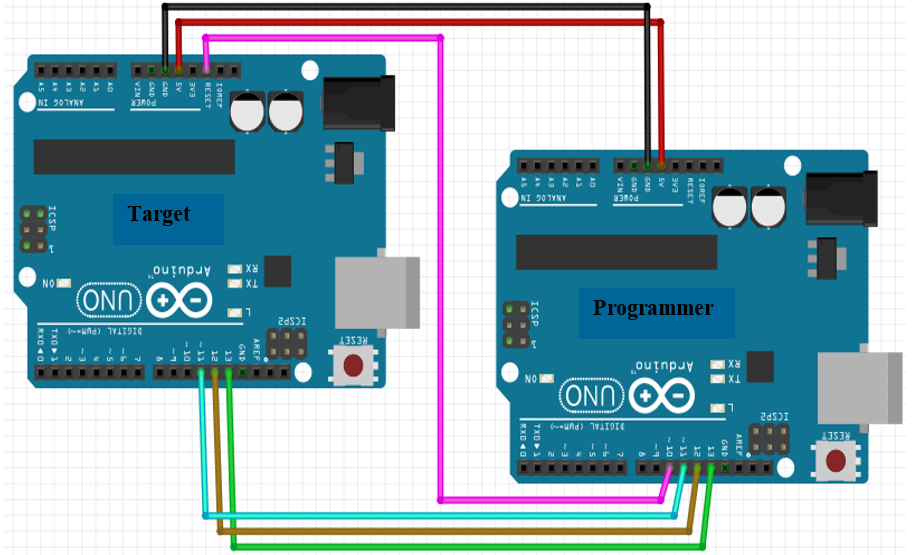
\includegraphics[scale=0.6]{EXP_03_Images/fig1.png}
    \end{center}
    \begin{center} {Figure 1. LED blinking circuit}\end{center}
\noindent \textbf{A) LED blinking with Arduino in TinkerCAD}\\
\vspace{-8mm}
\begin{enumerate}
    \item Components required for LED blinking in tinkercad are-LED (any color of your preference), 1 k$\Omega$ resistor, Bread Board, Arduino. Fig 2. shows the reference circuit which we are going to implement. Write the code in the code section as given in fig.3. Make sure you have defined pin13 (or any pin you have chosen) as OUTPUT throughout the program.
    
    \begin{center} 
    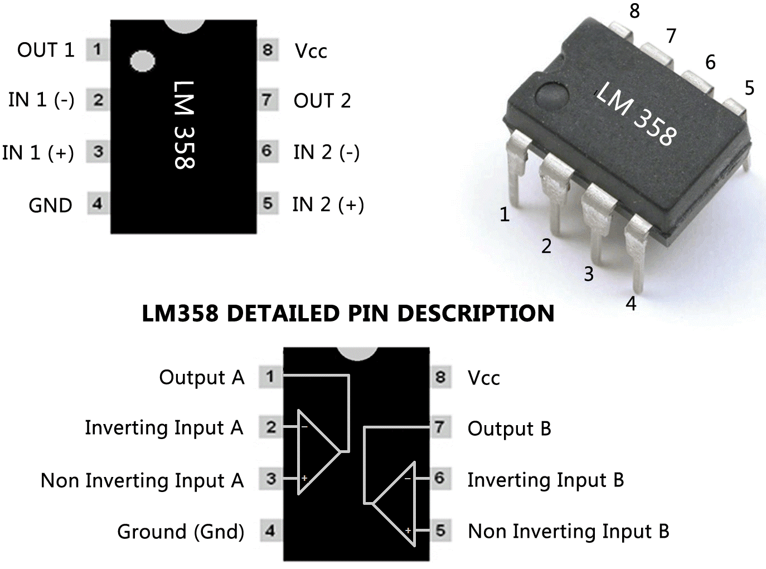
\includegraphics[scale=0.8]{EXP_03_Images/fig2.png}
    \end{center}
    \begin{center} {Figure 2. Components connection}\end{center}
    
    \begin{center} 
    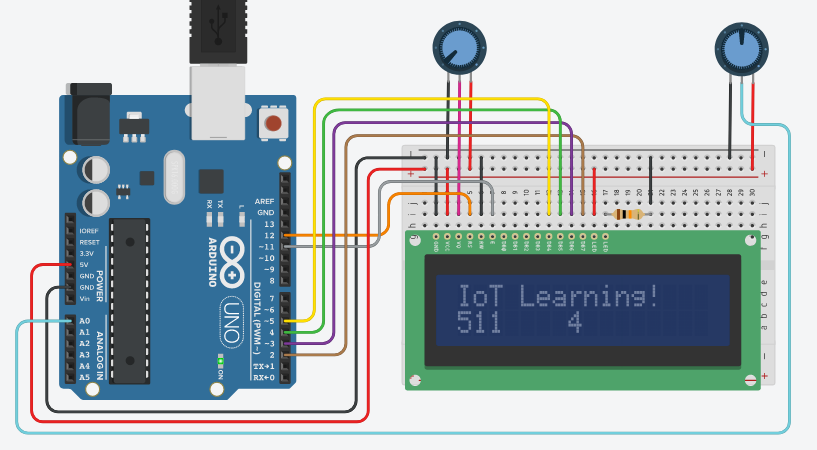
\includegraphics[scale=0.9]{EXP_03_Images/fig3.png}
    \end{center}
    \begin{center} {Figure 3. Code written in code editor }\end{center}
    
\vspace{2cm}
 \item Explanation of the code above: \\[3pt]
 An Arduino program generally has two sections: \textbf{void setup ()} and \textbf{void loop ()}:
    \begin{itemize}
      \item \textbf{void setup ()}: This section is used to initialize variables, pin modes, set the serial baud rate, start using libraries, etc. The software only goes through this section once after each power-up. The \textbf{setup ()} is a function in Arduino programming language (APL) used to declare configuration statements for the microcontroller ports. The \textbf{setup ()} function is called at the starting of the program and performs all the initialization. It contains multiple statements written inside parentheses.
      
      \item \textbf{void loop ():} This section is the part of the code that loops back onto itself and is the central part of the code. The \textbf{loop ()} is another predefined function responsible for indefinitely executing statements written inside its parentheses. This function enables the microcontroller (or Arduino board) to do a set of actions as long as it is ON. In our code, those actions are turn LED ON and OFF at certain time intervals.
      
      \item \textbf{pinmode():} It is essential that while programming with a microcontroller, we need to configure different microcontroller ports/pins as \textbf{INPUT} sources or \textbf{OUTPUT}. To configure Digital Pin 13 as OUTPUT, we must write the instruction \textbf{PinMode (13, OUTPUT)}.
      
      \item \textbf{digitalWrite():} To write data to a particular microcontroller port in the Arduino board. For this purpose, there is a keyword instruction called \textbf{HIGH} in APL. So we need to write an instruction \textbf{digitalWrite (13, HIGH)}. This instruction, when executed by the microcontroller, will supply +5 volts at Pin 13. This voltage will power the LED, and it will turn ON. Now to turn the LED OFF, we need to disconnect the voltage supply given at Pin 13. There is a keyword instruction named \textbf{LOW} in APL for this purpose. Write an instruction \textbf{digitalWrite (13, LOW)}, and we cut off supply at Pin 13. This instruction will turn the LED OFF. Now we need to be \textbf{setting a time interval} between ON and OFF time. Let's consider a 1-second time delay between ON and OFF time. 
      \item \textbf{delay() :}The function called \textbf{delay ()} is there in APL to setting time delay. We need to write the desired delay in \textbf{milliseconds} as an argument in the delay function. To get a 1-second delay, we should write \textbf{delay(1000)}; this will impart a delay of 1000 milliseconds between LED ON and OFF time.
   \end{itemize}
\end{enumerate}

\noindent \textbf{B)	Physical Realization - Hardware Setup:}

\noindent Follow the circuit diagram as given in fig. 1 and hook up the components on the breadboard, as shown in fig. 2. The LED's positive (+Ve) terminal is connected to one end of the resistor, and the other is connected to Digital Pin13. The negative (-Ve) terminal of the LED is connected to the ground. The resistor can be replaced with different values. It only changes the intensity of the LED. Note that it should be at least 100 ohms. Too large of a resistor can decrease the intensity too much, and with too low resistance, the LED can burn due to excess flow of current unbearable by LED.\\[6pt]
\noindent \textbf{Software Setup:}

    \begin{center} 
    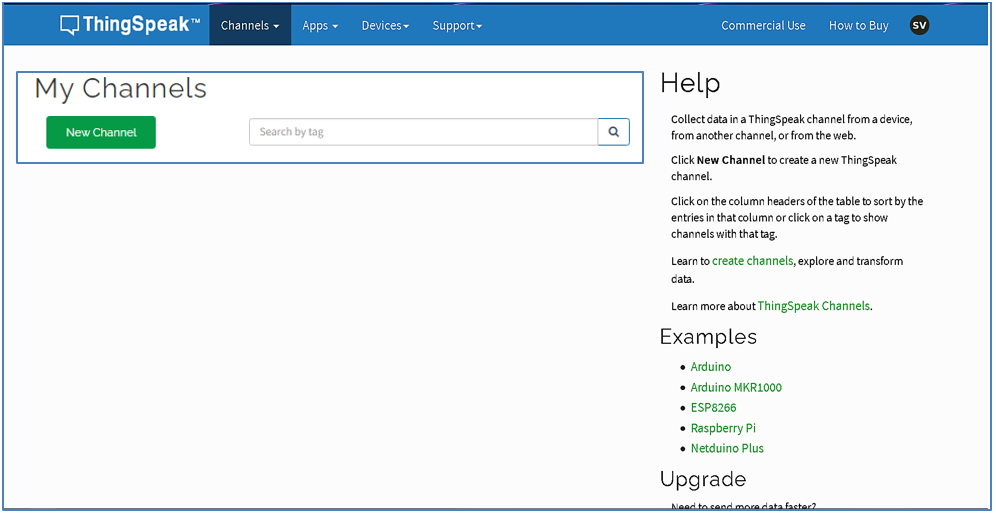
\includegraphics[scale=1]{EXP_03_Images/fig4.png}
    \end{center}
    \begin{center} {Figure 4. Software Setup}\end{center}

\noindent For setup and installation of IDE, check the Appendix. After setting up the IDE, open the Arduino IDE software on your computer. Coding in the Arduino IDE will control your circuit. Open the new sketch File by clicking New. We will write our code here. Blinking LED code is same as shown in figure 3.\par

\noindent Once the code is ready, the Arduino board is prepared to communicate with your PC and vice versa. Instructions will be sent to the Arduino board from your PC. For uploading the program from your PC to the Arduino board via the Arduino IDE, two steps need to be followed. The first step is \textbf{compiling}, and the second step is called \textbf{uploading}. Before that, connect the board to the PC and complete the following steps:

\begin{itemize}
\setlength\itemsep{-0.3em}
\item Select the board - Select the Arduino board type in the IDE. To choose the board, find Tools on the menu bar. Choose the option \textbf{"Board"} and select the correct Arduino board, Arduino UNO, as shown in fig.5.
\begin{center} 
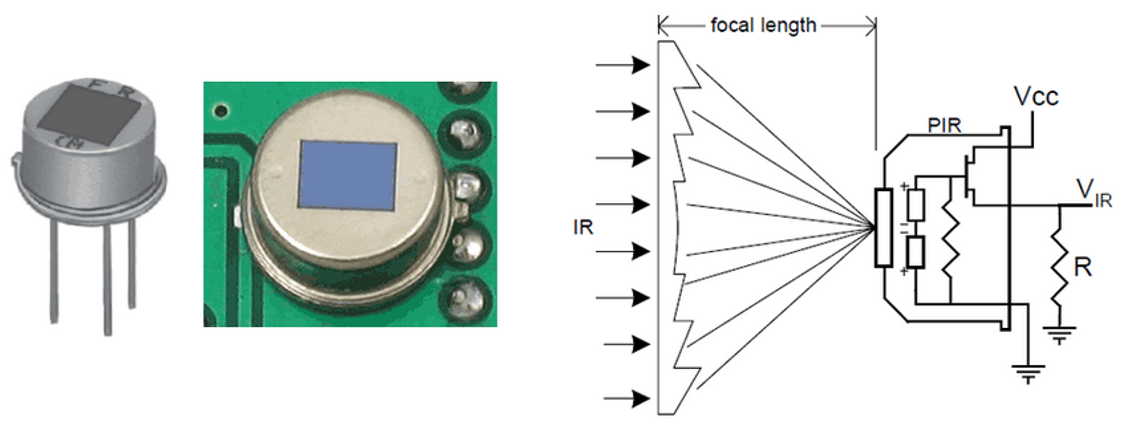
\includegraphics[scale=0.7]{EXP_03_Images/fig5.png}
\end{center}
\begin{center} {Figure 5. Arduino Board selection}\end{center}

\item Select the correct port-The port number is assigned to the board automatically if the proper driver has been installed. To select the correct port, go to \textbf{Tools$\rightarrow$Serial Port} and select the port number, shown in fig.6. 
\begin{center} 
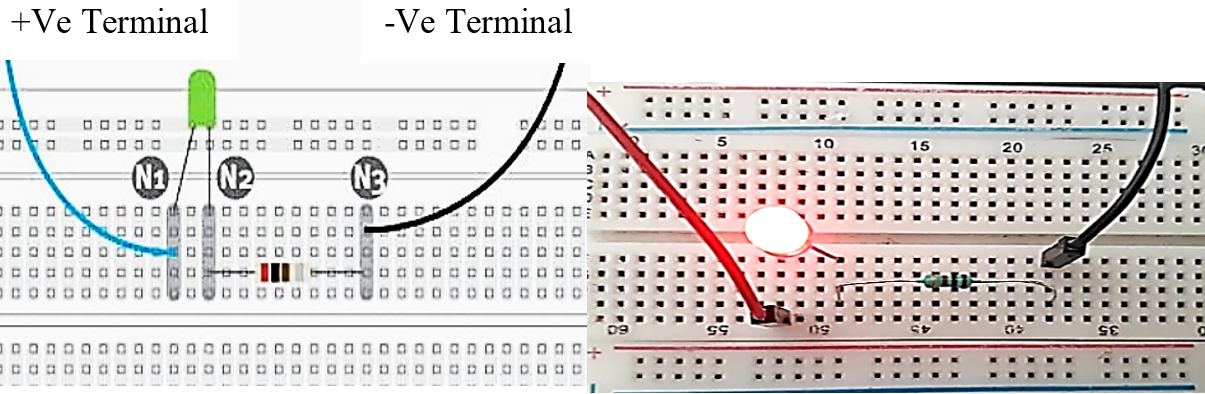
\includegraphics[scale=0.7]{EXP_03_Images/fig6.png}
\end{center}
\begin{center} {Figure 6. Selecting the port}\end{center}
\noindent Now that the proper port and board are selected, we can send the code to the Arduino. Save the code before the below steps:\\
\item \textbf{Compiling - } Compiling is the process of converting the code in Arduino IDE to another form which is only understood by the microcontroller in your Arduino board. In the Arduino IDE, compiling is called \textbf{"verify"}. So click the verify button in your IDE (see the button with tick mark just below the menu bar).

\begin{center} 
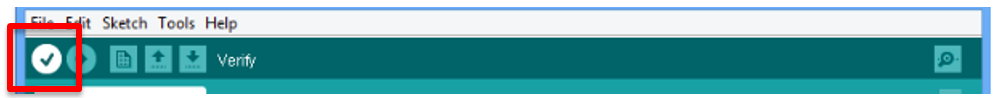
\includegraphics[scale=0.5]{EXP_03_Images/fig7.png}
\end{center}
\begin{center} {Figure 7.Verify on Arduino}\end{center}

\item \textbf{Uploading - }In this step, we will upload the verified/compiled code in Arduino IDE to the Arduino board. So press the \textbf{"upload"} button (see the button with the right arrow mark). A hit on the "upload" button will begin the process of burning the compiled program to the microcontroller on your connected Arduino board. Depending on the size of your code, this will take a few minutes. If you look on your Arduino Uno board, you will be able to see the 2 LEDs blinking near \textbf{Tx} and \textbf{Rx}. This blinking indicates the successful communication between your PC and the Arduino board. If the program has been uploaded successfully on your Arduino board, you will see a message like \textbf{"Done Uploading"}. If the uploading process was not successful, you would see an error message accordingly.  
\begin{center} 

\includegraphics[scale=0.5]{EXP_03_Images/fig8.png}
\end{center}
\begin{center} {Figure 8.Upload on Arduino}\end{center}
After the upload is done, the LED connected to the board is now blinking at the rate of 1 second.
\end{itemize}

\setlength{\parindent}{0eM}
\textbf{\large REFERENCES:}
\vspace{-6mm}
\begin{enumerate}
\setlength\itemsep{-0.3em}
\item  \href{https://www.electronicshub.org/getting-started-with-esp32/}{Arduino-Guide}
\item  \href{https://www.arduino.cc/en/Guide}{Arduino Pinout}
\item  \href{https://circuitsboards.blogspot.com/1969/12/arduino-uno-pinout-board.html?m=1}{Javatpoint-arduino-blinking}
\item  \href{https://www.javatpoint.com/arduino-blinking-multiple-leds-using-loop}{Learn.sparkfun-what-is-a-pull-up-resistor}
\item  \href{https://www.totalphase.com/support/articles/200349156-I2C-Background}{Totalphase.com-I2C-Background}
\item  \href{https://www.corelis.com/education/tutorials/spi-tutorial}{Corelis-SPI-tutorial}
\item  \href{https://stackoverflow.com/tags/uart/info }{Stackoverflow-UART}
\item  \href{https://www.arduino.cc/en/Main/ArduinoBoardUnoSMD }{Arduino - ArduinoBoardUnoSMD}
\item  \href{https://www.pcboard.ca/wavgat-arduino-uno-r3}{Arduino Uno R3 from Wavgat (pcboard.ca)}

\end{enumerate}

\textbf{\large CONCEPT DRILLS:}\\[3pt]
Connect RGB LED with Arduino and keep blinking the Red, Green, and Blue LED one after another at an interval of 2 seconds continuously.\\ 
RGB LEDs have three internal LEDs (Red, Green, and Blue) having one common anode or cathode and three other leads, each for Red, Green, and Blue. In our kit, the RGB LED has a common cathode as shown in the fig. 9 .\\
The RGB LEDs can produce almost any color output. In order to produce different kinds of colors, we need to set the intensity of each internal LED and combine the three color outputs. In later experiments, we can do it using PWM.\\

\begin{center} 
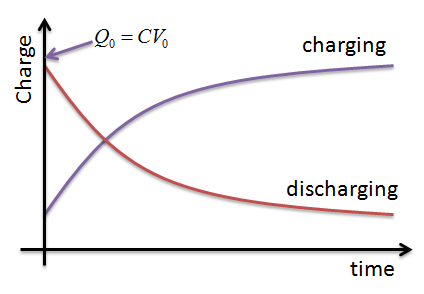
\includegraphics[scale=0.8]{EXP_03_Images/fig9.png}
\end{center}
\begin{center} {Figure 9.Common cathode RGB LED}\end{center}


\end{justify}
\end{document}